\documentclass{beamer}

\usetheme{Madrid} % Or choose another theme like Berlin, Warsaw, Singapore, etc.
\usecolortheme{default}

\usepackage{graphicx} % For including images
\usepackage{listings} % For code listings
\usepackage{textcomp} % For symbols like \textrightarrow

% Define code listing styles
\lstdefinestyle{customc}{
  language=C++,
  basicstyle=\scriptsize\ttfamily,
  keywordstyle=\color{blue},
  commentstyle=\color{green!70!black},
  stringstyle=\color{red},
  showstringspaces=false,
  breaklines=true,
  frame=tb,
  numbers=left,
  numberstyle=\tiny\color{gray},
}

\lstdefinestyle{custompy}{
  language=Python,
  basicstyle=\scriptsize\ttfamily,
  keywordstyle=\color{blue},
  commentstyle=\color{green!70!black},
  stringstyle=\color{red},
  showstringspaces=false,
  breaklines=true,
  frame=tb,
  numbers=left,
  numberstyle=\tiny\color{gray},
}

\lstdefinestyle{custommermaid}{
  language=Mermaid, % Assuming a simple text-based 'language' for mermaid
  basicstyle=\scriptsize\ttfamily,
  keywordstyle=\color{purple},
  breaklines=true,
  frame=tb,
}


\title{VisionVault: An Enhanced Wearable Camera System}
\subtitle{From Manual Capture to Automatic Auditory Descriptions}
\author{Analysis based on Project Files}
\date{\today}
\institute{Project Overview}

\begin{document}

% --- Title Frame ---
\begin{frame}
  \titlepage
\end{frame}

% --- Table of Contents ---
\begin{frame}{Outline}
  \tableofcontents
\end{frame}

% --- Introduction Section ---
\section{Introduction}

\begin{frame}{What is VisionVault?}
  \begin{columns}[T] % Align columns at the top
    \begin{column}{0.6\textwidth}
      \textbf{Core Idea:} An innovative project integrating an ESP32-CAM on goggles to capture and document moments.
      \vspace{1em}
      \begin{itemize}
        \item Transforms how moments are captured/documented.
        \item Allows users to stream live video.
        \item Capture images and generate descriptions via AI.
        \item Aims for hands-free operation.
      \end{itemize}
       \vspace{1em}
       \textbf{Applications:}
       \begin{itemize}
        \item Personal memory archival.
        \item Remote surveillance.
        \item Assistive technology.
      \end{itemize}
    \end{column}
    \begin{column}{0.4\textwidth}
      \centering
      \includegraphics[width=\linewidth]{"vision vault.jpeg"} \\ % Assuming image is in assets folder relative path needed or same folder
      \tiny Demo Image Placeholder
    \end{column}
  \end{columns}
\end{frame}

\begin{frame}[fragile]{Initial Concept: Key Components}
 \frametitle{Original Workflow (ESP32 \textrightarrow Python \textrightarrow Console)}
    \begin{itemize}
        \item \textbf{ESP32-CAM (`camera-feed.ino`):} Connects to WiFi, configures camera, streams MJPEG video via HTTP.
        \item \textbf{Python Script (`take-pic.py`):} Runs on host PC, connects to ESP32 stream, displays feed using OpenCV.
        \item \textbf{Manual Capture:} User presses 'c' key on the host PC.
        \item \textbf{AI Description:} Captured image (`captured\_image.jpg`) sent to Google Gemini API.
        \item \textbf{Output:} Description printed to the host PC console.
    \end{itemize}

    \vspace{0.5em}
    \textbf{Trigger Example (Original `take-pic.py`):}
    \begin{lstlisting}[style=custompy, firstnumber=58]
        # Check for key presses
        key = cv2.waitKey(1) & 0xFF

        # Save the image when 'c' is pressed
        if key == ord('c'):
            filename = f"captured_image.jpg"
            cv2.imwrite(filename, frame)
            print(f"Image saved as {filename}")
            # Create a separate thread to handle content generation
            threading.Thread(target=generate_content).start()

        #Press 'q' to quit the video display
        if key == ord('q'):
            break
    \end{lstlisting}
\end{frame}

% --- Enhancement Section ---
\section{Enhancements and New Workflow}

\begin{frame}{Motivation for Enhancement}
    \frametitle{Limitations of Initial Concept}
    \begin{itemize}
        \item Requires user interaction on the host PC (keyboard press).
        \item Not truly hands-free or mobile.
        \item Output is only text on the console.
        \item \textbf{Accessibility Challenge:} How does a visually impaired user know \textit{when} to press 'c'?
    \end{itemize}
    \vspace{1em}
    \textbf{Goals for Enhancement:}
    \begin{itemize}
        \item Create a mobile interface (React Native).
        \item Provide auditory feedback (Text-to-Speech).
        \item Enable automatic, periodic descriptions.
        \item Add user controls via the mobile app.
        \item Improve robustness and add security.
        \item Optimize API usage (Scene Change Detection).
    \end{itemize}
\end{frame}

\begin{frame}{Enhanced Workflow Overview}
  \frametitle{Mobile App \textrightarrow Python Server \textrightarrow TTS}
    Based on `WORKFLOW.md`:
    \begin{itemize}
        \item \textbf{ESP32-CAM:} Unchanged (streams video).
        \item \textbf{Python Backend Server:}
            \begin{itemize}
                \item Fetches stream continuously (with reconnection).
                \item Runs WebSocket Server (WSS) for mobile app communication.
                \item Manages client state (active/inactive, interval).
                \item \textbf{Automatic Mode:} Periodically checks for scene changes. If changed, sends frame to API, broadcasts description to active clients.
                \item Handles commands from app (`start`, `stop`, `set\_interval`, `describe\_now`).
            \end{itemize}
         \item \textbf{React Native Mobile App:}
            \begin{itemize}
                \item Connects to Python Server (WSS, with reconnection).
                \item UI: Start/Stop, Interval config, Describe Now, History, Status.
                \item Sends commands to server.
                \item Receives descriptions/errors.
                \item Provides TTS output and Haptic feedback.
            \end{itemize}
    \end{itemize}
\end{frame}

% --- Architecture Section ---
\section{System Architecture}

\begin{frame}{Enhanced System Architecture}
    \frametitle{Overall Component Interaction}
    \begin{figure}
        \centering
        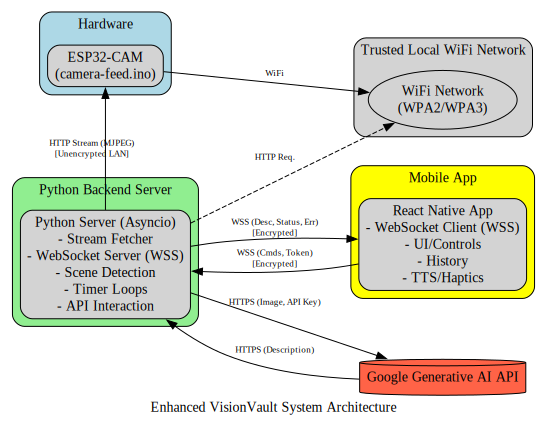
\includegraphics[width=0.95\textwidth]{Sys_Arch.png} % Use generated PNG
        \caption{High-level view of components and communication protocols.}
    \end{figure}
\end{frame}

\begin{frame}{Python Backend Server Internals}
    \frametitle{Modular Design}
     \begin{figure}
        \centering
        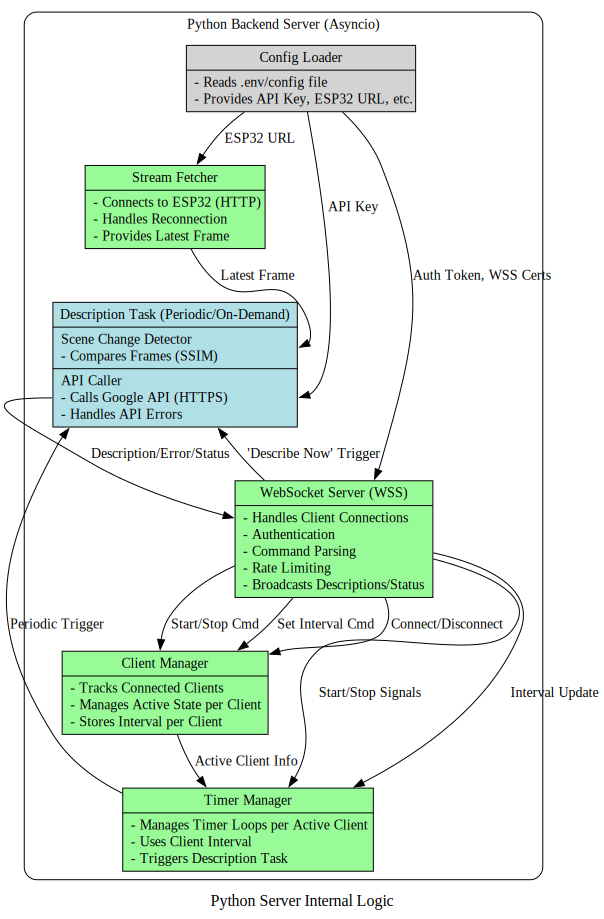
\includegraphics[height=0.8\textheight, width=0.8\textwidth, keepaspectratio]{Python_Server_Internal_Logic_Diagram.png} % Use generated PNG
        \caption{Key internal modules and data flow within the Python server.}
    \end{figure}
\end{frame}

\begin{frame}{Mobile App UI Flow}
    \frametitle{User Interaction States}
     \begin{figure}
        \centering
        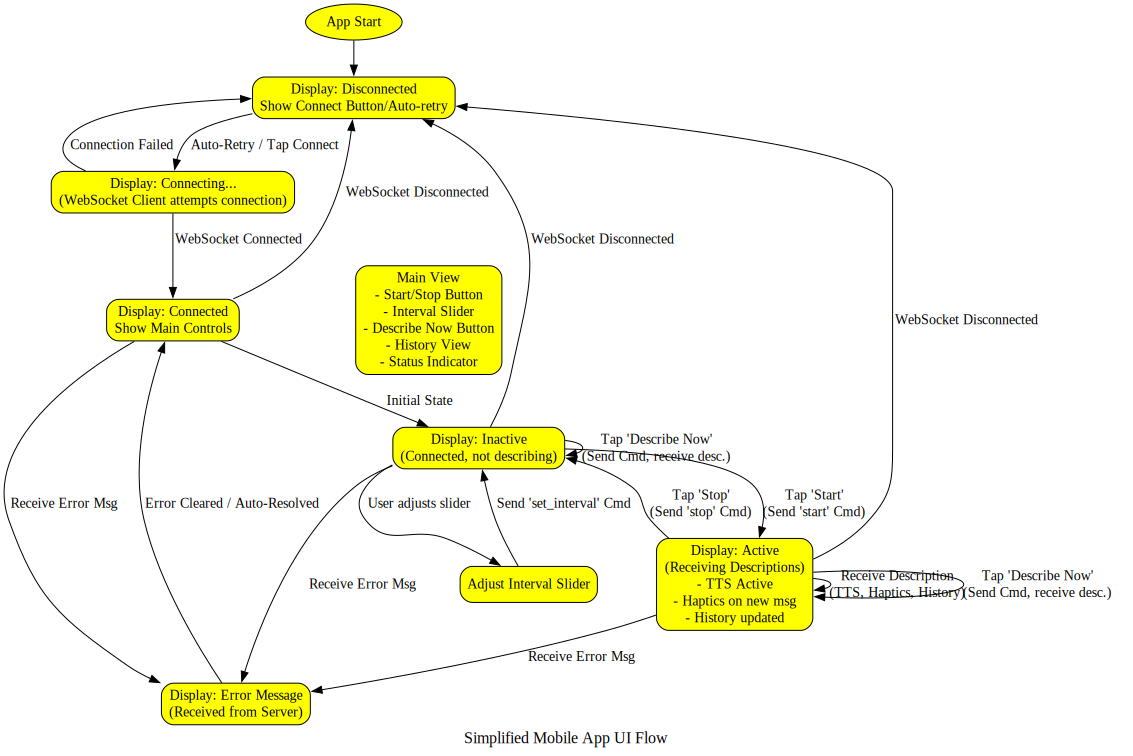
\includegraphics[height=0.8\textheight, width=\textwidth, keepaspectratio]{Mobile_App_UI_Flow_Diagram.png} % Use generated PNG
        \caption{Simplified state transitions within the React Native application.}
    \end{figure}
\end{frame}

% --- Core Logic Section ---
\section{Core Logic and Flows}

\begin{frame}{Sequence: Automatic Description}
    \frametitle{How Continuous Description Works}
    \begin{figure}
        \centering
        % Mermaid source can't be directly rendered, use the PNG
        \includegraphics[width=\textwidth, height=0.8\textheight, keepaspectratio]{sequenceDiagram.png}
        \caption{Sequence of events for automatic description triggered by timer.}
    \end{figure}
\end{frame}

\begin{frame}{Algorithm: Scene Change Detection}
    \frametitle{Optimizing API Calls}
     \begin{figure}
        \centering
        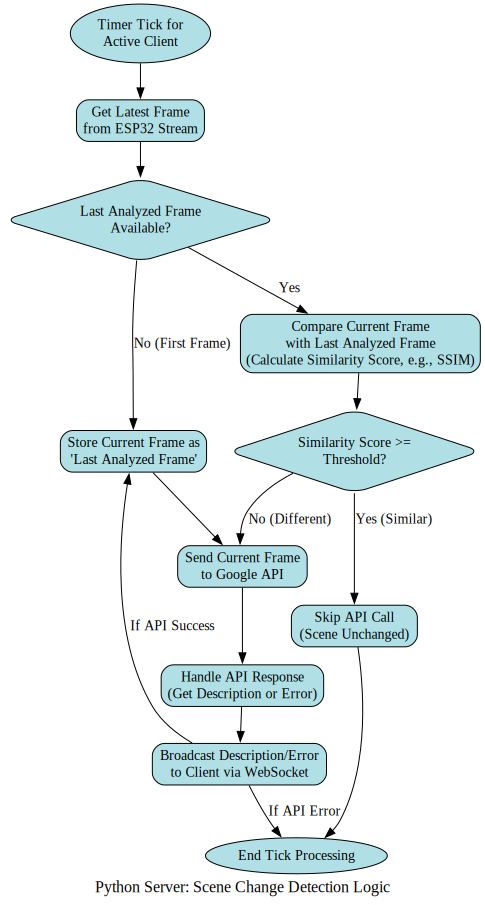
\includegraphics[height=0.8\textheight, width=0.6\textwidth, keepaspectratio]{Scene_Change_Detection_Logic_Flowchart.png} % Use generated PNG
        \caption{Flowchart for deciding whether to call the AI API based on frame similarity.}
    \end{figure}
\end{frame}

% --- Technology & Code Section ---
\section{Technology and Code}

\begin{frame}{Technology Stack}
    \frametitle{Key Technologies Used}
    Based on `WORKFLOW.md`:
    \begin{itemize}
        \item \textbf{Hardware:} ESP32-CAM
        \item \textbf{Video Streaming:} MJPEG over HTTP
        \item \textbf{Backend:} Python 3 with `asyncio`, `websockets`, `aiohttp`/`requests`, `opencv-python`, `scikit-image` (for SSIM), `google-generativeai`, `python-dotenv`.
        \item \textbf{Frontend:} React Native (JavaScript/TypeScript)
        \item \textbf{Communication:} Secure WebSockets (WSS)
        \item \textbf{AI:} Google Generative AI (Gemini API)
        \item \textbf{Output:} Text-to-Speech (TTS) Library (React Native)
        \item \textbf{Feedback:} Haptics API (React Native)
    \end{itemize}
\end{frame}

\begin{frame}[fragile]{Code Snippet: ESP32-CAM Setup}
  \frametitle{From `camera-feed.ino` (Camera Configuration)}
    \begin{lstlisting}[style=customc, firstnumber=88, numbers=none]
  // ... (Pin definitions) ...

  camera_config_t config;
  config.ledc_channel = LEDC_CHANNEL_0;
  config.ledc_timer = LEDC_TIMER_0;
  config.pin_d0 = Y2_GPIO_NUM;
  // ... (Assign all camera pins) ...
  config.pin_xclk = XCLK_GPIO_NUM;
  config.pin_pclk = PCLK_GPIO_NUM;
  config.pin_vsync = VSYNC_GPIO_NUM;
  config.pin_href = HREF_GPIO_NUM;
  config.pin_sscb_sda = SIOD_GPIO_NUM;
  config.pin_sscb_scl = SIOC_GPIO_NUM;
  config.pin_pwdn = PWDN_GPIO_NUM;
  config.pin_reset = RESET_GPIO_NUM;
  config.xclk_freq_hz = 20000000;
  config.pixel_format = PIXFORMAT_JPEG; // Important for MJPEG stream

  // Frame size and quality based on PSRAM
  if(psramFound()){
    config.frame_size = FRAMESIZE_VGA; // Or other size
    config.jpeg_quality = 10; // 0-63 lower means higher quality
    config.fb_count = 2;
  } else {
    config.frame_size = FRAMESIZE_QQVGA;
    config.jpeg_quality = 15;
    config.fb_count = 1;
  }

  // Camera init
  esp_err_t err = esp_camera_init(&config);
  if (err != ESP_OK) { // Error handling
    Serial.printf("Camera init failed with error 0x%x", err);
    return;
  }
  // ... (WiFi connection and start server) ...
    \end{lstlisting}
\end{frame}

% --- Security Section ---
\section{Security Aspects}

\begin{frame}{Security Considerations}
    \frametitle{Risks and Mitigations (Trusted LAN Focus)}
     Highlights from `WORKFLOW.md`:
     \begin{itemize}
        \item \textbf{Network:} Assumes trusted WiFi (WPA2/WPA3). Public networks are risky.
        \item \textbf{ESP32 Stream (HTTP):} Unencrypted. Rely on WiFi security. HTTPS on ESP32 is challenging.
        \item \textbf{WebSocket (WSS):} \textit{Mitigation:} Use Secure WebSockets (`wss://`) with TLS certificates to encrypt app-server communication.
        \item \textbf{Authentication:} \textit{Mitigation:} Implement token-based authentication for WebSocket clients to prevent unauthorized access/commands.
        \item \textbf{API Key:} \textit{Mitigation:} Store securely (e.g., `.env` file, environment variables). Secure the host machine.
        \item \textbf{DoS:} \textit{Mitigation:} Implement rate limiting on WebSocket commands/connections on the server.
        \item \textbf{Input Validation:} \textit{Mitigation:} Sanitize all commands/data received from the mobile app on the server.
        \item \textbf{Resource Management:} Ensure server cleans up resources on client disconnect.
     \end{itemize}
\end{frame}

\begin{frame}{Security Flow: WSS Authentication}
    \frametitle{Connecting Securely}
     \begin{figure}
        \centering
        % Mermaid source can't be directly rendered, use the PNG
        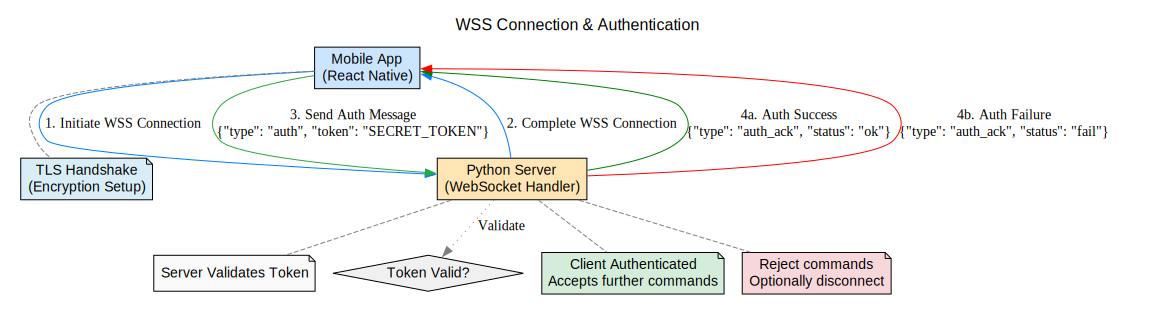
\includegraphics[width=0.9\textwidth, height=0.7\textheight, keepaspectratio]{Security_Flow_Diagram.png}
        \caption{Sequence for establishing a secure WebSocket connection with token authentication.}
    \end{figure}
\end{frame}


% --- Conclusion Section ---
\section{Conclusion}

\begin{frame}{Summary}
    \frametitle{VisionVault - Enhanced}
    \begin{itemize}
        \item Evolved from a simple capture tool to an assistive technology concept.
        \item Utilizes ESP32-CAM for video streaming.
        \item Python backend manages stream, AI interaction, and app communication via WSS.
        \item React Native app provides user control, history, and auditory (TTS) / tactile (Haptic) feedback.
        \item Incorporates efficiency (scene change detection) and security (WSS, Auth) measures.
        \item Provides a robust framework for real-time environmental description.
    \end{itemize}
     \vspace{1em}
     \textbf{Next Steps would involve actual implementation based on these designs.}
\end{frame}


\end{document}
